45. \begin{figure}[ht!]
\center{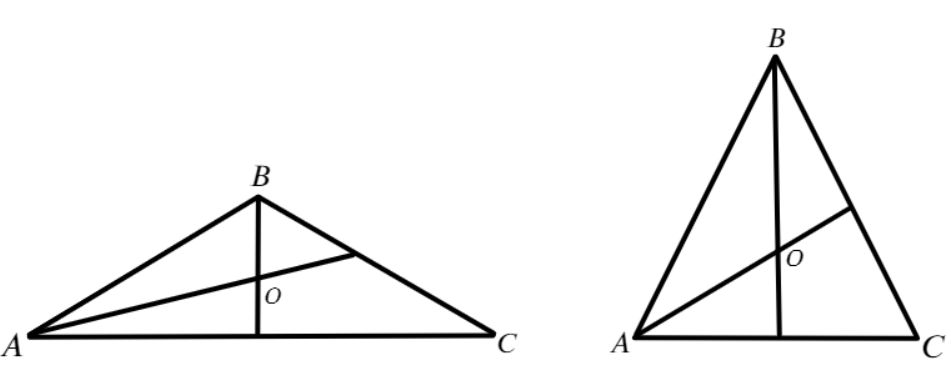
\includegraphics[scale=0.35]{g45.png}}
\end{figure}\\
Возможны два случая: в треугольнике угол при вершине равен $5x,$ а углы при основании по $2x$ и наоборот, угол при вершине равен $2x,$ а углы при основании --- по $5x.$ В первом случае $5x+2\cdot2x=180^\circ,\ 9x=180^\circ,\ x=20^\circ,$ значит угол при вершине равен $5\cdot20^\circ=100^\circ,$ а углы при основании равны $2\cdot20^\circ=40^\circ.$ Тогда $\angle AOB=180^\circ-\frac{1}{2}\angle A-\frac{1}{2}\angle B=180^\circ-20^\circ-50^\circ=110^\circ.$ Так как углом между прямыми является наименьший из углов, образованных этими прямыми, угол между биссектрисами в этом случае равен $180^\circ-110^\circ=70^\circ.$ Во втором случае $2x+2\cdot5x=180^\circ,\ 12x=180^\circ,\ x=15^\circ,$ значит угол при вершине равен $2\cdot15^\circ=30^\circ,$ а углы при основании равны $5\cdot15^\circ=75^\circ.$
Тогда $\angle AOB=180^\circ-\frac{1}{2}\angle A-\frac{1}{2}\angle B=180^\circ-15^\circ-37^\circ30'=127^\circ30'.$ Так как углом между прямыми является наименьший из углов, образованных этими прямыми, угол между биссектрисами в этом случае равен $180^\circ-127^\circ30'=52^\circ30'.$
ewpage

oindent46. \begin{figure}[ht!]
\center{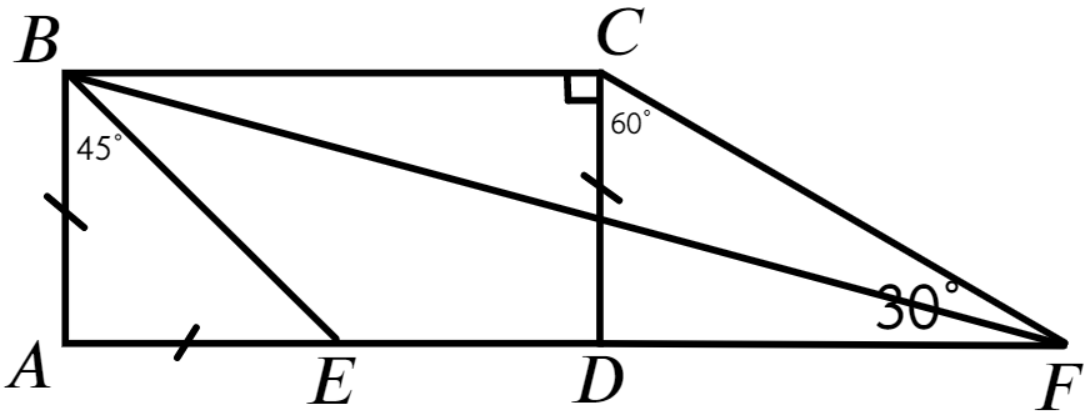
\includegraphics[scale=0.35]{g46.png}}
\end{figure}\\
Так как $AE=\frac{1}{2}AD=\frac{1}{2}BC=AB,$ треугольник $ABE$ является равнобедренным и поэтому $\angle ABE=(180^\circ-90^\circ):2=45^\circ.$ В прямоугольном треугольнике $CDF$ угол $DCF$ равен $90^\circ-30^\circ=60^\circ$ и катет $CD$ лежит напротив угла в $30^\circ,$ поэтому $CF=2CD=2AB=BC.$ Тогда треугольник $BCF$ является равнобедренным и угол при его вершине $C$ равен $90^\circ+60^\circ=150^\circ,$ а поэтому $\angle FBC=(180^\circ-150^\circ):2=15^\circ.$ Таким образом, $\angle EBF=90^\circ-45^\circ-15^\circ=30^\circ.$\\
